% !TeX root = ..\main.tex
\section{Thiết kế cơ sở dữ liệu}
\par Nhóm lựa chọn kiến trúc Microservice cho hệ thống, với việc chia ra các service nhỏ và mỗi service có một database riêng phục vụ cho nghiệp vụ của riêng service đó, nên ở đây các database được thiết kế riêng lẻ cho từng service.

\subsection{ERD/EERD}
\subsubsection{Service Khách hàng}
\begin{figure}[!htp]
	\begin{center}
		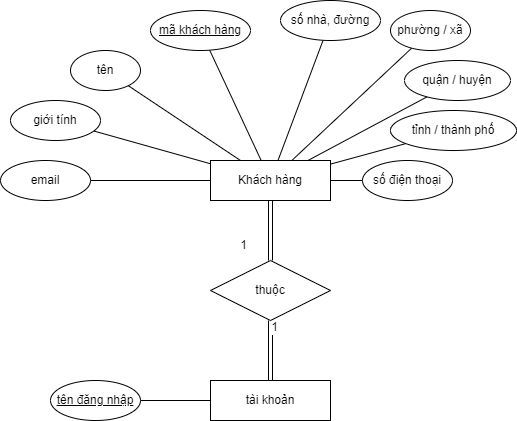
\includegraphics[width=0.7\textwidth]{img/database/erd/eerd-customer.png}
		\newline
		\caption{ERD cho database của service Khách hàng}
	\end{center}
\end{figure}

\par Database của service Khách hàng bao gồm hai thực thể là Khách hàng và Tài khoản của khách hàng. Thực thể khách hàng chứa các thông tin cá nhân của khách hàng, bao gồm các thuộc tính:
\begin{itemize}
	\item Mã khách hàng: thuộc tính khóa, là mã của khách hàng.
	\item Tên: Là tên của khách hàng.
	\item Giới tính: Là giới tính của khách hàng.
	\item Email: Là email của khách hàng.
	\item Số điện thoại: Là số điện thoại của khách hàng.
	\item Số nhà, đường: Là địa chỉ sô nhà, đường của khách hàng ở.
	\item Phường / xã: Là địa chỉ phường / xã của khách hàng ở.
	\item Quận / huyện: Là địa chỉ quận / huyện của khách hàng ở.
	\item Tỉnh / thành phố: Là địa chỉ tỉnh / thành phố của khách hàng ở.
\end{itemize}

\par Thực thể Tài khoản của khách hàng bao gồm các thuộc tính:
\begin{itemize}
	\item Tên đăng nhập: tên đăng nhập của tài khoản của khách hàng.
\end{itemize}

\par Khách hàng và Tài khoản có mối quan hệ thuộc, đây là mối quan hệ bắt buộc, 1-1: một khách hàng chỉ thuộc 1 tài khoản và 1 tài khoản chỉ dùng cho 1 khách hàng.

\subsubsection{Service Giỏ hàng}
\begin{figure}[!htp]
	\begin{center}
		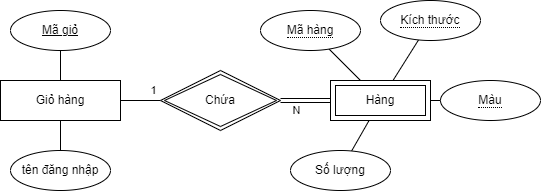
\includegraphics[width=0.7\textwidth]{img/database/erd/eerd-cart.png}
		\newline
		\caption{ERD cho database của service Giỏ hàng}
	\end{center}
\end{figure}

\par Database của service Giỏ hàng bao gồm hai thực thể là Giỏ hàng và Hàng trong giỏ hàng. Thực thể Giỏ hàng chứa thông tin về giỏ hàng, bao gồm các thuộc tính:
\begin{itemize}
	\item Mã giỏ hàng: thuộc tính khóa, là mã của giỏ hàng.
	\item Mã khách hàng: là mã khách hàng của khách hàng chủ của giỏ hàng đó.
	\item Số lượng món: là thuộc tính dẫn xuất, số lượng loại sản phẩm có trong giỏ hàng.
\end{itemize}

\par Thực thể Hàng trong giỏ hàng chứa thông tin của mặt hàng trong trong giỏ hàng đó. Thực thể này bao gồm các thuộc tính:
\begin{itemize}
	\item Mã hàng: thuộc tính khóa, là mã của loại hàng đó.
	\item Kích thước: thuộc tính khóa, là kích thước của loại hàng đó.
	\item Màu: thuộc tính khóa, là màu sắc của loại hàng đó.
\end{itemize}

\par Giỏ hàng và Hàng có mối quan hệ chứa, Mối quan hệ là M-N. Giỏ hàng tham gia vào mối quan hệ với ràng buộc tham gia không bắt buộc: Giỏ hàng có thể chứa hàng hoặc không, có thể chứa hàng với số lượng khác nhau. Hàng tham gia vào mối quan hệ với ràng buộc tham gia không bắt buộc, một hàng có thể có hoặc không thuộc giỏ hàng nào. Mối quan hệ này có các thuộc tính:
\begin{itemize}
	\item Số lượng: số lượng của món hàng có trong giỏ hàng.
\end{itemize}

\subsubsection{Service Đơn hàng của khách hàng}
\begin{figure}[!htp]
	\begin{center}
		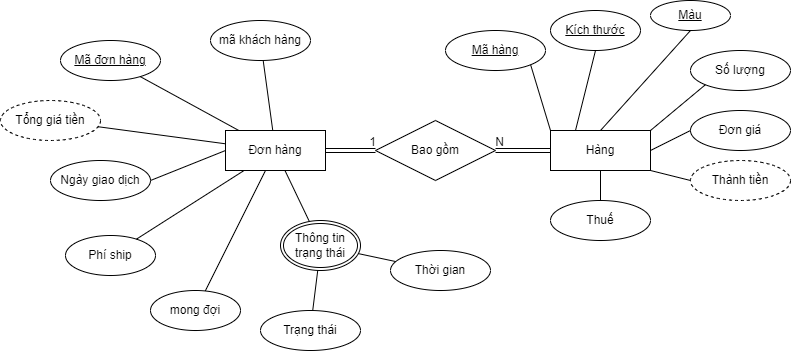
\includegraphics[width=1\textwidth]{img/database/erd/eerd-customer-order.png}
		\newline
		\caption{ERD cho database của service Đơn hàng của khách hàng}
	\end{center}
\end{figure}

\par Database của service Đơn hàng của khách hàng bao gồm hai thực thể là Đơn hàng và Hàng trong đơn hàng. Thực thể Đơn hàng chứa thông tin về đơn hàng, bao gồm các thuộc tính:
\begin{itemize}
	\item Mã đơn hàng: thuộc tính khóa, là mã của đơn hàng.
	\item Mã khách hàng: là mã khách hàng của khách hàng chủ của đơn hàng đó.
	\item Ngày giao dịch: là ngày thực hiện giao dịch của đơn hàng.
	\item Phí ship: là phí vận chuyển của đơn hàng.
	\item Mong đợi: là thời gian ước tính để giao đơn hàng.
	\item Tổng giá tiền: là thuộc tính dẫn xuất, là tổng giá tiền của đơn hàng.
	\item Thông tin trạng thái: là thuộc tính đa trị, là trạng thái của đơn hàng, bao gồm 2 thuộc tính con là Trạng thái và Thời gian. Trạng thái là trạng thái của đơn hàng và thời gian là thời điểm xảy ra trạng thái của đơn hàng.
\end{itemize}

\par Thực thể Hàng trong đơn hàng chứa thông tin của mặt hàng trong trong đơn hàng đó. Thực thể này bao gồm các thuộc tính:
\begin{itemize}
	\item Mã hàng: thuộc tính khóa, là mã của loại hàng đó.
	\item Kích thước: thuộc tính khóa, là kích thước của loại hàng đó.
	\item Màu: thuộc tính khóa, là màu sắc của loại hàng đó.
	\item Số lượng: là số lượng của loại hàng trong đơn hàng.
	\item Đơn giá: là giá tiền của loại hàng trong đơn hàng.
	\item Thuế: là thuế được thu trên loại hàng đó trong đơn hàng.
	\item Thành tiền: là thuộc tính dẫn xuất, giá tiền cuối cùng được tính cho loại hàng đó trong đơn hàng.
\end{itemize}

\par Đơn hàng và Hàng có mối quan hệ Bao gồm, đây là quan hệ bắt buộc, Mối quan hệ là 1-N: đơn hàng bắt buộc có hàng, và có thể có nhiều hàng; hàng trong đơn hàng bắt buộc phải thuộc về một đơn hàng, và chỉ thuộc về duy nhất một đơn hàng.

\subsubsection{Service Sự kiện}
\begin{figure}[!htp]
	\begin{center}
		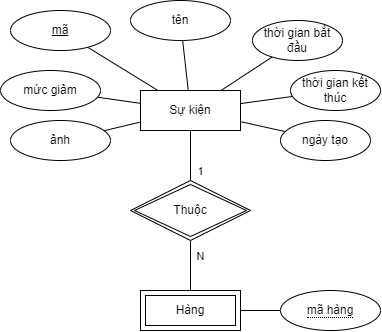
\includegraphics[width=0.6\textwidth]{img/database/erd/eerd-event.png}
		\newline
		\caption{ERD cho database của service Sự kiện}
	\end{center}
\end{figure}

\par Database của service Sự kiện bao gồm hai thực thể là Sự kiện và Hàng. Thực thể Sự kiện chứa thông tin về sự kiện, bao gồm các thuộc tính:
\begin{itemize}
	\item Mã sự kiện: thuộc tính khóa, là mã của sự kiện.
	\item Tên: là của sự kiện.
	\item Giảm giá: là giá trị giảm giá của sự kiện đối với các mặt hàng trong sự kiện.
	\item Thời gian bắt đầu: là thời gian bắt đầu sự kiện.
	\item Thời gian kết thúc: là thời gian kết thúc sự kiện.
\end{itemize}

\par Thực thể Hàng trong sự kiện chứa thông tin của mặt hàng trong trong sự kiện đó. Thực thể này bao gồm các thuộc tính:
\begin{itemize}
	\item Mã hàng: thuộc tính khóa, là mã của loại hàng đó.
\end{itemize}

\par Sự kiện và Hàng có mối quan hệ có, mối quan hệ là M-N: sự kiện có thể có nhiều hàng, ít hàng hoặc không có hàng; hàng trong cũng có thể thuộc không hoặc ít hoặc nhiều sự kiện.

\subsubsection{Service Hàng hóa}
\begin{figure}[!htp]
	\begin{center}
		\includegraphics[width=1\textwidth]{img/database/erd/shop_online-hàng.png}
		\newline
		\caption{ERD cho database của service Hàng hóa}
	\end{center}
\end{figure}

\par Database của service Hàng hóa bao gồm hai thực thể là Hàng hóa và Hàng trong kho. Thực thể hàng hóa chỉ thông tin các mặt hàng được bán, bao gồm các thuộc tính:
\begin{itemize}
	\item Mã hàng: thuộc tính khóa, là mã của mặt hàng.
	\item Kích thước: thuộc tính khóa, là kích thước của mặt hàng.
	\item Màu: thuộc tính khóa, là màu của mặt hàng.
	\item Tên hàng: là tên của mặt hàng.
	\item Lứa tuổi: là lứa tuổi phù hợp của mặt hàng.
	\item Giới tính: là giới tính phù hợp của mặt hàng.
	\item Nhà sản xuất: là nhà sản xuất của mặt hàng.
	\item Hình ảnh: thuộc tính đa trị, bao gồm các hình ảnh của mặt hàng.
	\item Được bán: cho biết mặt hàng có đang được mở bán hay không.
	\item Đơn giá: giá tiền cho một đơn vị của mặt hàng.
	\item Mô tả: thông tin thêm về mặt hàng.
	\item Loại: thể loại của mặt hàng.
	\item Số lượng hiện tại: thuộc tính dẫn xuất, là số lượng còn tồn hiện tại của mặt hàng.
\end{itemize}

\par Thực thể Hàng trong kho chỉ thông tin của mặt hàng trong một kho nào đó. Thực thể này bao gồm các thuộc tính:
\begin{itemize}
	\item Mã kho: thuộc tính khóa, là mã của kho chứa hàng đó.
	\item Số lượng: số lượng hàng đó còn trong kho.
	\item Ngày tạo: ngày mặt hàng lần đầu vào kho.
	\item Ngày thay đổi: ngày hàng trong kho có sự thay đổi.
\end{itemize}

\par Hàng hóa và Hàng trong kho có mối quan hệ Bao gồm, đây là mối quan hệ bắt buộc, 1-N: hàng hóa bắt buộc phải nằm trong kho, và một mặt hàng có thể nằm ở nhiều kho; hàng trong kho bắt buộc thuộc về một mặt hàng, và chỉ thuộc về duy nhất một mặt hàng.

\subsubsection{Service Đơn hàng}
\begin{figure}[!htp]
	\begin{center}
		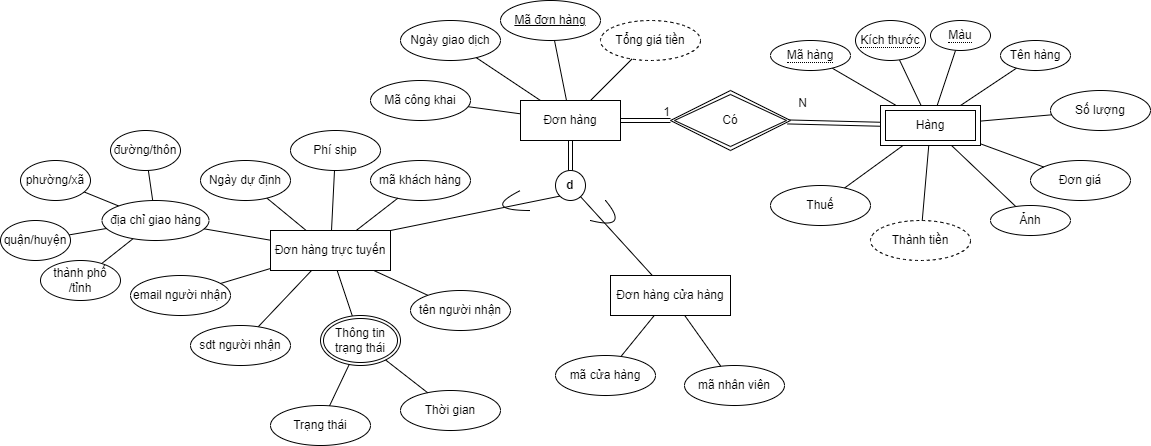
\includegraphics[width=1\textwidth]{img/database/erd/shop_online-đơnhàng.png}
		\newline
		\caption{ERD cho database của service Đơn hàng}
	\end{center}
\end{figure}

\par Database của service Đơn hàng bao gồm các thực thể Đơn hàng và Hàng hóa, chỉ các hàng hóa trong đơn hàng. Đơn hàng được cụ thể hóa xuống Đơn hàng online và Đơn hàng cửa hàng.
\par Thực thể Đơn hàng gồm các thuộc tính:
\begin{itemize}
	\item Mã đơn hàng: thuộc tính khóa, chỉ mã của đơn hàng.
	\item Ngày giao dịch: ngày thực hiện giao dịch mua hàng và sinh ra đơn hàng.
	\item Tổng giá tiền: thuộc tính dẫn xuất, là tổng giá tiền của đơn hàng.
\end{itemize}

\par Thực thể Đơn hàng online có thêm các thuộc tính:
\begin{itemize}
	\item Mã khách hàng: là mã khách hàng đã mua hàng online.
	\item Phí ship: giá tiền cho việc vận chuyển đơn hàng.
	\item Mong đợi: ngày giao hàng mong đợi.
	\item Thông tin trạng thái: thuộc tính phức hợp, bao gồm các thông tin Trạng thái và Thời gian chỉ các trạng thái và thời gian đạt đến trạng thái đó của đơn hàng.
\end{itemize}

\par Thực thể Đơn hàng cửa hàng có thêm thuộc tính:
\begin{itemize}
	\item Mã cửa hàng: mã cửa hàng bán hàng trong đơn hàng.
\end{itemize}

\par Thực thể Hàng bao gồm các thuộc tính:
\begin{itemize}
	\item Mã hàng: thuộc tính khóa, là mã của mặt hàng trong đơn hàng.
	\item Kích thước: thuộc tính khóa, là kích thước của hàng trong đơn hàng.
	\item Màu: thuộc tính khóa, là màu của hàng trong đơn hàng.
	\item Số lượng: số lượng hàng đã mua trong đơn hàng.
	\item Đơn giá: giá tiền một đơn vị của hàng trong đơn hàng.
	\item Thuế: giá tiền thuế của hàng trong đơn hàng.
	\item Thành tiền: thuộc tính dẫn xuất, là tổng giá tiền (đơn giá * số lượng) + thuế.
\end{itemize}

\par Đơn hàng và Hàng có quan hệ Bao gồm, đây là quan hệ bắt buộc, 1-N: đơn hàng bắt buộc có hàng, và có thể có nhiều hàng; hàng trong đơn hàng bắt buộc phải thuộc về một mặt hàng, và chỉ thuộc về duy nhất một mặt hàng.

\subsubsection{Service Kho}
\begin{figure}[!htp]
	\begin{center}
		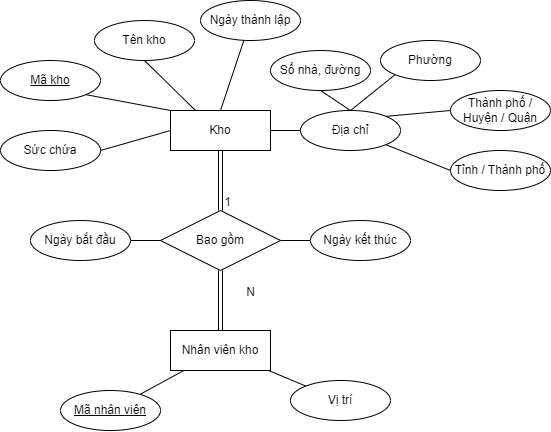
\includegraphics[width=1\textwidth]{img/database/erd/shop_online-Kho.png}
		\newline
		\caption{ERD cho database của service Kho}
	\end{center}
\end{figure}

\par Database của service Kho bao gồm thực thể Kho và thực thể Nhân viên kho. Thực thể Kho bao gồm các thuộc tính:
\begin{itemize}
	\item Mã kho: thuộc tính khóa, là mã của kho.
	\item Tên kho: tên của kho.
	\item Ngày thành lập: ngày mà kho đi vào sử dụng.
	\item Địa chỉ: thuộc tính kết hợp, bao gồm các thuộc tính Số nhà, đường, Phường, Thành phố / Quận / Huyện, Tỉnh / Thành phố.
	\item Sức chứa: sức chứa hàng tối đa của kho.
	\item Còn lại: thuộc tính dẫn xuất, chỉ sức chứa còn lại mà kho có thể chứa hàng thêm.
\end{itemize}

\par Thực thể Nhân viên kho bao gồm các thuộc tính:
\begin{itemize}
	\item Mã nhân viên: thuộc tính khóa, là mã của nhân viên làm việc ở kho.
\end{itemize}

\par Kho và nhân viên kho có mối quan hệ Bao gồm là mối quan hệ bắt buộc, M-N: kho bắt buộc có nhân viên, và có thể có nhiều nhân viên làm việc; nhân viên buộc phải làm việc ở ít nhất một kho, và có thể làm việc ở nhiều kho. Mối quan hệ này có các thuộc tính:
\begin{itemize}
	\item Ngày bắt đầu: ngày nhân viên bắt đầu làm việc tại kho đó.
	\item Ngày kết thúc: ngày nhân viên nghỉ làm việc tại kho đó.
\end{itemize}

\par Mỗi kho có một quản lý, nên kho và nhân viên quản lý có mối quan hệ Được quản lý bởi. Mối quan hệ là M-N. Kho tham gia vào mối quan hệ với ràng buộc tham gia bắt buộc: kho phải có quản lý, và theo thời gian có nhiều quản lý theo từng thời gian khác nhau. Quản lý - cũng là nhân viên kho, tham gia vào mối quan hệ với ràng buộc tham gia không bắt buộc, một nhân viên không cần phải làm quản lý, và qua thời gian có thể làm quản lý ở nhiều kho. Mối quan hệ này có các thuộc tính:
\begin{itemize}
	\item Ngày bắt đầu: ngày quản lý bắt đầu làm việc tại kho đó.
	\item Ngày kết thúc: ngày quản lý nghỉ làm việc tại kho đó.
\end{itemize}

\subsubsection{Service chi nhánh}
\begin{figure}[!htp]
	\begin{center}
		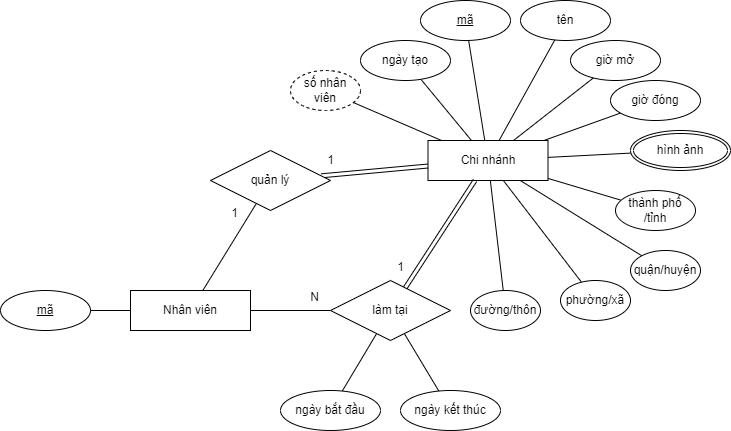
\includegraphics[width=1\textwidth]{img/database/erd/branch.png}
		\newline
		\caption{ERD cho database của service chi nhánh}
	\end{center}
\end{figure}

Database của service chi nhánh bao gồm hai thực thể là Nhân viên và chi nhánh. Thực thể chi nhánh chứa thông tin về chi nhánh:
\begin{itemize}
	\item mã: thuộc tính khóa, là mã của chi nhánh.
	\item tên: Tên chi nhánh.
	\item ngày tạo: Ngày tạo chi nhánh.
	\item giờ mở: Giờ mở cửa mổi ngày của chi nhánh.
	\item giờ đóng: Giờ đóng cửa mổi ngày của chi nhánh.
	\item hình ảnh: Hình ảnh minh họa chi nhánh.
	\item đường/thôn: Tên đường của chi nhánh.
	\item phường/xã: Phường xã của chi nhánh.
	\item quận/huyện: Quận, huyện của chi nhánh.
	\item thành phố /tỉnh: Tỉnh, thành phố của chi nhánh
\end{itemize}

Thực thể Nhân viên chỉ chứa một vài thông tin nhân viên:
\begin{itemize}
	\item mã: thuộc tính khóa, là mã của nhân viên.
\end{itemize}

Chi nhánh và nhân viên có mối quan hệ Làm tại và Quản lý: Mỗi chi nhánh đều phải có ít nhất một nhân viên và một quản lý. Mối quan hệ Bao gồm có các thông tin:
\begin{itemize}
	\item ngày bắt đầu: ngày bắt đầu làm việc tại chi nhánh của nhân viên.
	\item ngày kết thúc: ngày kết thúc làm việc tại chi nhánh của nhân viên.
\end{itemize}


\subsubsection{Service tài khoản}
\begin{figure}[!htp]
	\begin{center}
		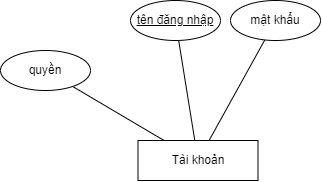
\includegraphics[width=5cm]{img/database/erd/account.png}
		\newline
		\caption{ERD cho database của service tài khoản}
	\end{center}
\end{figure}

Database của service tài khoản chỉ có thực thể tài khoản chứa thông tin về tài khoản:
\begin{itemize}
	\item tên đăng nhập: Thuộc tính khóa, là tên đăng nhập của tài khoản.
	\item mật khẩu: Mật khẩu của tài khoản.
	\item quyền: Quyền của tài khoản.
\end{itemize}


\subsubsection{Service nhân viên}
\begin{figure}[!htp]
	\begin{center}
		\includegraphics[width=1\textwidth]{img/database/erd/staff.png}
		\newline
		\caption{ERD cho database của service nhân viên}
	\end{center}
\end{figure}

Database của service nhân viên chứa các thực thể Nhân viên, Bản yêu cầu, Tài khoản, Bản điểm danh. Thực thể Nhân viên bao gồm các thông tin của nhân viên:
\begin{itemize}
	\item mã: thuộc tính khóa, là mã của nhân viên.
	\item tên: Tên nhân viên.
	\item cccd: Căn cước công dân chi nhánh
	\item vị trí: Vị trí làm việc trong cửa hàng
	\item lương: Mức lương của nhân viên
	\item ngày vào: Ngày được nhận vào làm.
	\item sdt: Số điện thoại của nhân viên.
	\item email: Email của nhân viên.
	\item đường/thôn: Tên đường của nhân viên.
	\item phường/xã: Phường xã của nhân viên.
	\item quận/huyện: Quận, huyện của nhân viên.
	\item thành phố /tỉnh: Tỉnh, thành phố của nhân viên
\end{itemize}

Thực thể Bản yêu cầu chứa thông tin về yêu cầu thêm, xóa nhân viên:
\begin{itemize}
	\item mã: thuộc tính khóa, là mã của yêu cầu.
	\item ngày yêu cầu: Ngày tạo yêu cầu
	\item loại yêu cầu: Loại của yêu cầu là thêm hay xóa
	\item trạng thái: Trạng thái của yêu cầu đang chờ, được duyệt hoặc hủy bỏ
\end{itemize}

Thực thể Bản điểm danh chứa thông tin về hoạt động điểm danh của nhân viên:
\begin{itemize}
	\item ngày: thuộc tính khóa, là ngày làm việc của nhân viên.
	\item thời gian vào: Thời gian bắt đầu vào làm trong ngày của nhân viên
	\item thời gian ra: Thời gian kết thúc làm trong ngày của nhân viên
	\item thời gian làm: Thời gian làm việc trong ngày của nhân viên
\end{itemize}

Thực thể Tài khoản chỉ chứa thông tin về tên tài khoản của nhân viên

Nhân viên và Bản yêu cầu có mối quan hệ Thuộc về: Mỗi bản yêu cầu đều phải thuộc về một nhân viên

Nhân viên và Tài khoản có mối quan hệ Có: Chỉ có các nhân viên cấp quản lý mới sở hữu tài khoản

Nhân viên và Bản điểm danh cầu có mối quan hệ Điểm danh: Tât cả bản điểm danh đều phải có nhân viên


\subsubsection{Service thống kê}
\begin{figure}[!htp]
	\begin{center}
		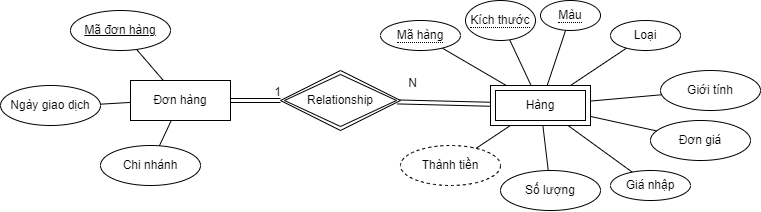
\includegraphics[width=1\textwidth]{img/database/erd/Statistic.png}
		\newline
		\caption{ERD cho database của service thống kê}
	\end{center}
\end{figure}

Database của service chi nhánh bao gồm hai thực thể là Đơn hàng và hàng. Thực thể đơn hàng chứa thông tin về các đơn hàng:
\begin{itemize}
	\item Mã đơn hàng: thuộc tính khóa, là mã của đơn hàng.
	\item Ngày giao dịch: Ngày tạo đơn hàng.
	\item mã cửa hàng: Nơi tạo đơn hàng.
\end{itemize}

Thực thể Hàng chỉ chứa một vài thông tin của hàng hóa được bán:
\begin{itemize}
	\item Mã hàng: thuộc tính khóa, là mã của món hàng.
	\item Kích thước: thuộc tính khóa, là kích thước của món hàng.
	\item Màu: thuộc tính khóa, là mã của món hàng.
	\item Loại: Loại của món hàng.
	\item Số lượng: Số lượng của món hàng trong đơn.
	\item Giới tính: Giới tính của món hàng.
	\item chi phí: Giá nhập của món hàng.
	\item đơn giá: Đơn giá bán ra của món hàng.
\end{itemize}

Đơn hàng và hàng có mối quan hệ bao gồm: Mỗi đơn hàng đều phải có ít nhất một món hàng và mỗi món hàng đều phải nằm trong ít nhất một đơn hàng:


\subsection{Ánh xạ}
\par Từ các ERD/EERD trên, chúng ta có các ánh xạ sau tương ứng với mỗi service.

\subsubsection{Service Khách hàng}
\begin{figure}[!htp]
	\begin{center}
		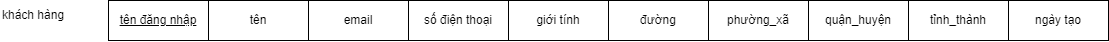
\includegraphics[width=1\textwidth]{img/database/mapping/mapping-customer.png}
		\newline
		\caption{Ánh xạ cho database của service Khách hàng}
	\end{center}
\end{figure}

Bảng dữ liệu Khách hàng trong service Khách hàng bao gồm các thuộc tính và kiểu dữ liệu như sau:
\begin{itemize}
	\item Mã khách hàng: string.
	\item Tên đăng nhập: string.
	\item Tên: string.
	\item Email: string.
	\item Số điện thoại: string.
	\item Giới tính: string.
	\item Đường: string.
	\item Phường\_xã: string.
	\item Quận\_huyện: string.
	\item Tỉnh\_thành: string.
\end{itemize}

\subsubsection{Service Giỏ hàng}
\begin{figure}[!htp]
	\begin{center}
		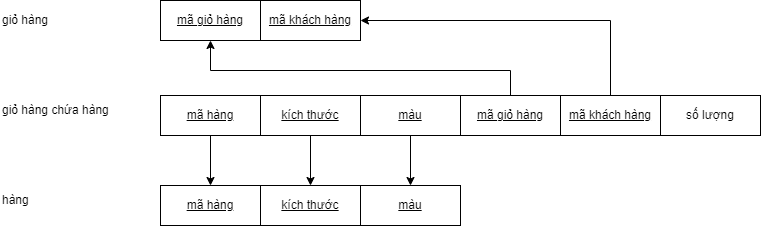
\includegraphics[width=1\textwidth]{img/database/mapping/mapping-cart.png}
		\newline
		\caption{Ánh xạ cho database của service Giỏ hàng}
	\end{center}
\end{figure}

Bảng dữ liệu Giỏ hàng trong service Giỏ hàng bao gồm các thuộc tính và kiểu dữ liệu như sau:
\begin{itemize}
	\item Mã giỏ hàng: string.
	\item Mã khách hàng: string.
	\item Số lượng: int.
	\item Mã hàng: string.
	\item Kích thước: string.
	\item Màu: string.
\end{itemize}

Bảng dữ liệu Hàng trong service Giỏ hàng bao gồm các thuộc tính và kiểu dữ liệu như sau:
\begin{itemize}
	\item Mã hàng: string.
	\item Kích thước: string.
	\item Màu: string.
\end{itemize}

\subsubsection{Service Đơn hàng của khách hàng}
\begin{figure}[!htp]
	\begin{center}
		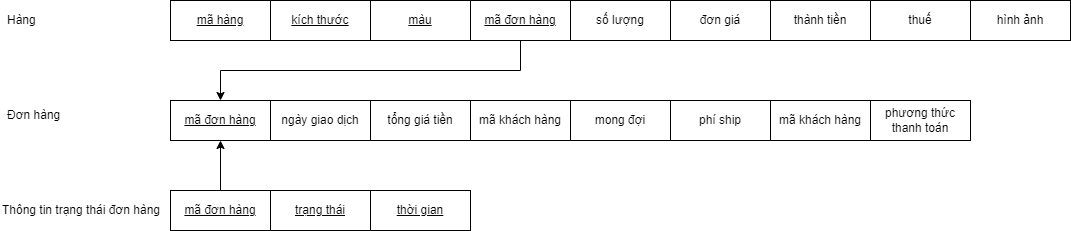
\includegraphics[width=1\textwidth]{img/database/mapping/mapping-customer-order.png}
		\newline
		\caption{Ánh xạ cho database của service Đơn hàng của khách hàng}
	\end{center}
\end{figure}

Bảng dữ liệu Hàng trong service Đơn hàng của khách hàng bao gồm các thuộc tính và kiểu dữ liệu như sau:
\begin{itemize}
	\item Mã hàng: string.
	\item Mã đơn hàng: string.
	\item Số lượng: int.
	\item Mã hàng: string.
	\item Kích thước: string.
	\item Màu: string.
	\item Đơn giá: int.
	\item Thành tiền: int.
	\item Thuế: int.
	\item Hình ảnh: string.
\end{itemize}

Bảng dữ liệu Đơn hàng trong service Đơn hàng của khách hàng bao gồm các thuộc tính và kiểu dữ liệu như sau:
\begin{itemize}
	\item Mã đơn hàng: string.
	\item Ngày giao dịch: string.
	\item Tổng giá tiền: int.
	\item Mã khách hàng: int.
	\item Mong đợi: string.
	\item Phí ship: int.
	\item Mã khách hàng: string.
	\item Phương thức thanh toán: string.
\end{itemize}

Bảng dữ liệu Thông tin trạng thái đơn hàng trong service Đơn hàng của khách hàng bao gồm các thuộc tính và kiểu dữ liệu như sau:
\begin{itemize}
	\item Mã đơn hàng: string.
	\item Trạng thái: string.
	\item Thời gian: datetime.
\end{itemize}

\subsubsection{Service Sự kiện}
\begin{figure}[!htp]
	\begin{center}
		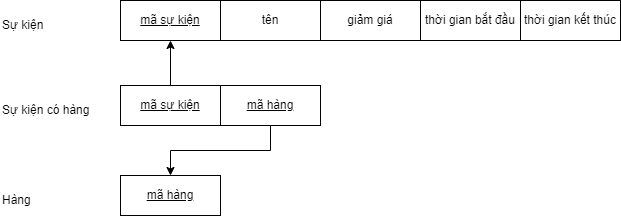
\includegraphics[width=0.8\textwidth]{img/database/mapping/mapping-event.png}
		\newline
		\caption{Ánh xạ cho database của service Sự kiện}
	\end{center}
\end{figure}

Bảng dữ liệu Sự kiện trong service Sự kiện bao gồm các thuộc tính và kiểu dữ liệu như sau:
\begin{itemize}
	\item Mã sự kiện: string.
	\item Tên: string.
	\item Giảm giá: int.
	\item Thời gian bắt đầu: datetime.
	\item Thời gian kết thúc: datetime.
\end{itemize}


Bảng dữ liệu Sự kiện có hàng trong service Sự kiện bao gồm các thuộc tính và kiểu dữ liệu như sau:
\begin{itemize}
	\item Mã sự kiện: string.
	\item Mã hàng: string.
\end{itemize}

\subsubsection{Service Hàng hóa}
\begin{figure}[!htp]
	\begin{center}
		\includegraphics[width=1\textwidth]{img/database/mapping/mapping-hàng.png}
		\newline
		\caption{Ánh xạ cho database của service Hàng hóa}
	\end{center}
\end{figure}

\subsubsection{Service Đơn hàng}
\begin{figure}[!htp]
	\begin{center}
		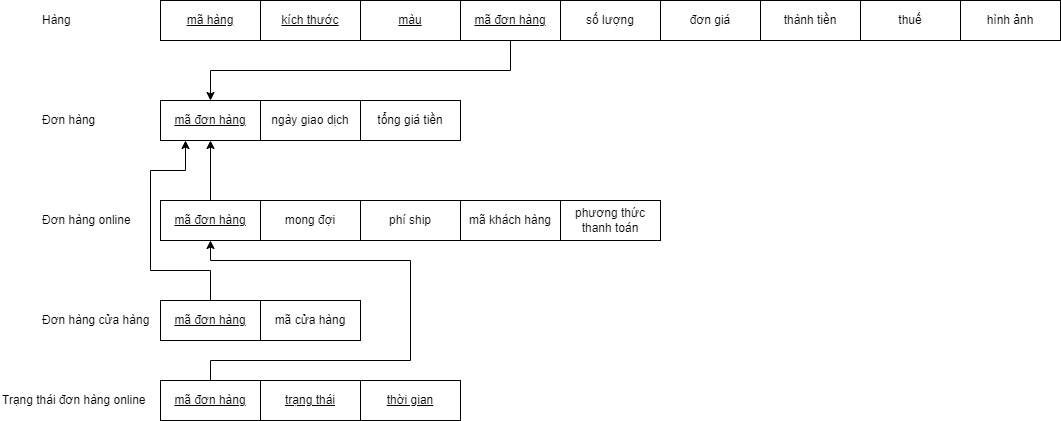
\includegraphics[width=1\textwidth]{img/database/mapping/mapping-đơnhàng.png}
		\newline
		\caption{Ánh xạ cho database của service Đơn hàng}
	\end{center}
\end{figure}

\subsubsection{Service Kho}
\begin{figure}[!htp]
	\begin{center}
		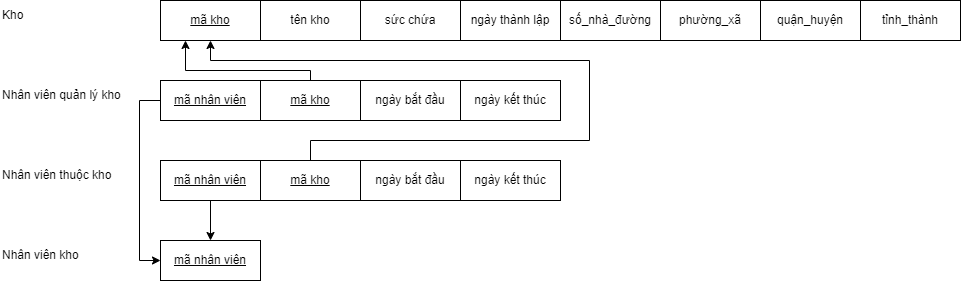
\includegraphics[width=1\textwidth]{img/database/mapping/mapping-kho.png}
		\newline
		\caption{Ánh xạ cho database của service Kho}
	\end{center}
\end{figure}

\subsubsection{Service chi nhánh}
\begin{figure}[!htp]
	\begin{center}
		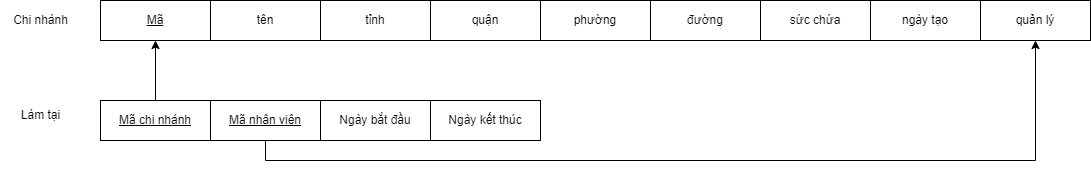
\includegraphics[width=1\textwidth]{img/database/mapping/branch.png}
		\newline
		\caption{Ánh xạ cho database của service chi nhánh}
	\end{center}
\end{figure}


\subsubsection{Service tài khoản}
\begin{figure}[!htp]
	\begin{center}
		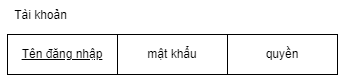
\includegraphics[width=5cm]{img/database/mapping/account.png}
		\newline
		\caption{Ánh xạ cho database của service tài khoản}
	\end{center}
\end{figure}

\subsubsection{Service nhân viên}
\begin{figure}[!htp]
	\begin{center}
		\includegraphics[width=1\textwidth]{img/database/mapping/staff.png}
		\newline
		\caption{Ánh xạ cho database của service nhân viên}
	\end{center}
\end{figure}


\subsubsection{Service thống kê}
\begin{figure}[!htp]
	\begin{center}
		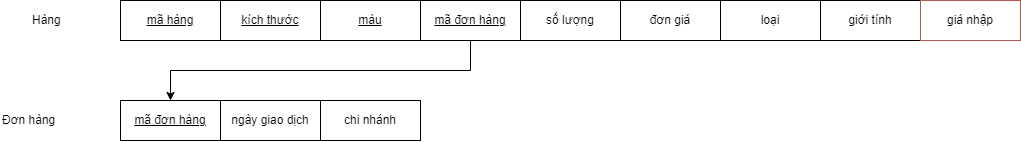
\includegraphics[width=1\textwidth]{img/database/mapping/Statistic.png}
		\newline
		\caption{Ánh xạ cho database của service thống kê}
	\end{center}
\end{figure}